\documentclass[10pt,a4paper,twocolumn,twoside]{article}
\usepackage[utf8]{inputenc}
\usepackage[catalan]{babel}
\usepackage{multicol}
\usepackage{graphicx}
\usepackage{fancyhdr}
\usepackage{times}
\usepackage{titlesec}
\usepackage{multirow}
\usepackage{lettrine}
\usepackage[top=2cm, bottom=1.5cm, left=2cm, right=2cm]{geometry}
\usepackage[figurename=Fig.,tablename=TAULA]{caption}
\captionsetup[table]{textfont=sc}

\author{\LARGE\sffamily Narcís Nogué Bonet}
\title{\Huge{\sffamily Aterratge autònom d'aeronaus d'ala fixa basat en visió}}
\date{}

\newcommand\blfootnote[1]{%
  \begingroup
  \renewcommand\thefootnote{}\footnote{#1}%
  \addtocounter{footnote}{-1}%
  \endgroup
}

%
%\large\bfseries\sffamily
\titleformat{\section}
{\large\sffamily\scshape\bfseries}
{\textbf{\thesection}}{1em}{}

\begin{document}

\fancyhead[LO]{\scriptsize NARCÍS NOGUÉ BONET}
\fancyhead[RO]{\thepage}
\fancyhead[LE]{\thepage}
\fancyhead[RE]{\scriptsize ATERRATGE AUTÒNOM D'AVIONS MODEL BASAT EN VISIÓ}

\fancyfoot[CO,CE]{}

\fancypagestyle{primerapagina}
{
   \fancyhf{}
   \fancyhead[L]{\scriptsize TFG EN ENGINYERIA INFORMÀTICA, ESCOLA D'ENGINYERIA (EE), UNIVERSITAT AUTÒNOMA DE BARCELONA (UAB)}
   \fancyfoot[C]{\scriptsize Juny de 2021, Escola d'Enginyeria (UAB)}
}

%\lhead{\thepage}
%\chead{}
%\rhead{\tiny EE/UAB TFG INFORMÀTICA: TÍTOL (ABREUJAT SI ÉS MOLT LLARG)}
%\lhead{ EE/UAB \thepage}
%\lfoot{}
%\cfoot{\tiny{February 2015, Escola d'Enginyeria (UAB)}}
%\rfoot{}
\renewcommand{\headrulewidth}{0pt}
\renewcommand{\footrulewidth}{0pt}
\pagestyle{fancy}

%\thispagestyle{myheadings}
\twocolumn[\begin{@twocolumnfalse}

%\vspace*{-1cm}{\scriptsize TFG EN ENGINYERIA INFORMÀTICA, ESCOLA D'ENGINYERIA (EE), UNIVERSITAT AUTÒNOMA DE BARCELONA (UAB)}

\maketitle

\thispagestyle{primerapagina}
%\twocolumn[\begin{@twocolumnfalse}
%\maketitle
%\begin{abstract}
\begin{center}
\parbox{0.915\textwidth}
{\sffamily
\textbf{Resum--}
Resum del projecte, màxim 10 línies. ........ ........... .......... ..  ... ..... .... ........ ........... .......... ..  ... ..... .... ........ ........... .......... ..  ... ..... .... ........ ........... .......... ..  ... ..... .... ........ ........... .......... ..  ... ..... .... ........ ........... .......... ..  ... ..... .... ........ ........... .......... ..  ... ..... .... ........ ........... .......... ..  ... ..... .... ........ ........... .......... ..  ... ..... .... ........ ........... .......... ..  ... ..... .... ........ ........... .......... ..  ... ..... .... .................. ..  ... ..... .... ........ ........... .......... ..  ... ..... .... ........ ........... .......... ..  ... ..... .... ........ ........... .......... ..  ... ..... .... ........ ........... .......... ..  ... ..... .... ........ ........... .......... ..  ... ..... .... ........ ........ .......... ..  ... . ........... .......... ..  ... ..... .... ........ ........... .......... ..  ... ..... .... ........ ........... .......... ..  ... ..... .... ........ ........... .......... ..  ... ........... ..  ... ..... .... ........ ........... .......... ..  ... ..... .... ........ ........... .......... ..  ... ..... .... ........ ........... .......... ..  ... ..... .... ........ ........... .......... ..  ... ..... .... ........ ........... .......... ..  ... ..... .... ........ ........... .......... ..  ... ..... .... ........ ........... .......... ..  ... ..... .... ........ ........... .......... ..  ... ..... .... 
\\
\\
\textbf{Paraules clau-- } Paraules clau del treball, màxim 2 línies . .... ........ ........... .......... ..  ... ..... .... ........ ........... .......... ..  ... ..... .... ........ ........... ................\\
\\
%\end{abstract}
%\bigskip
%\begin{abstract}
\bigskip
\\
\textbf{Abstract--} Versió en anglès del resum . ........ ........... .......... ..  ... ..... .... ........ ........... .......... ..  ... ..... .... ........ ........... .......... ..  ... ..... .... ........ ........... .......... ..  ... ..... .... ........ ........... .......... ..  ... ..... .... ........ ........... .......... ..  ... ..... .... ........ ........... .......... ..  ... ..... .... ........ ........... .......... ..  ... ..... .... ........ ........... .......... ..  ... ..... .... ........ ........... .......... ..  ... ..... .... ........ ........... .......... ..  ... ..... .... .................. ..  ... ..... .... ........ ........... .......... ..  ... ..... .... ........ ........... .......... ..  ... ..... .... ........ ........... .......... ..  ... ..... .... ........ ........... .......... ..  ... ..... .... ........ ........... .......... ..  ... ..... .... ........ ........ .......... ..  ... . ........... .......... ..  ... ..... .... ........ ........... .......... ..  ... ..... .... ........ ........... .......... ..  ... ..... .... ........ ........... .......... ..  ... ........... ..  ... ..... .... ........ ........... .......... ..  ... ..... .... ........ ........... .......... ..  ... ..... .... ........ ........... .......... ..  ... ..... .... ........ ........... .......... ..  ... ..... .... ........ ........... .......... ..  ... ..... .... ........ ........... .......... ..  ... ..... .... ........ ........... .......... ..  ... ..... .... ........ ........... .......... ..  ... ..... .... 
\\
\\
\textbf{Keywords-- } Versió en anglès de les paraules clau. .... ........ ........... .......... ..  ... ..... .... ........ ........... .......... ..  ... ..... .... ........ ........... .................. ..\\
}

\bigskip

{\vrule depth 0pt height 0.5pt width 4cm\hspace{7.5pt}%
\raisebox{-3.5pt}{\fontfamily{pzd}\fontencoding{U}\fontseries{m}\fontshape{n}\fontsize{11}{12}\selectfont\char70}%
\hspace{7.5pt}\vrule depth 0pt height 0.5pt width 4cm\relax}

\end{center}

\bigskip
%\end{abstract}
\end{@twocolumnfalse}]

\blfootnote{$\bullet$ E-mail de contacte: xxx@yyy.zzz}
\blfootnote{$\bullet$ Menció realitzada: Enginyeria de Computadors / Computació / Enginyeria del Software / Tecnologies de la Informació}
\blfootnote{$\bullet$ Treball tutoritzat per: nom i cognoms del tutor (departament)}
\blfootnote{$\bullet$ Curs 20xx/xx}

\section{Introducció - Context del treball}

\lettrine[lines=3]{C}{om} indica el títol, el meu Treball de Final de Grau consisteix a crear un
sistema de control autònom que sigui capaç d'aterrar un avió en una pista
d'aterratge utilitzant únicament una càmera i altres sensors bàsics com
acceleròmetres i giroscopis. Actualment la majoria de sistemes d'aterratge
autònom necessiten modificacions substancials de la pista d'aterratge per instal·lar
un sistema ILS (Instrument Landing System), dissenyat per permetre a una aeronau
aterrar de nit o en baixa visibilitat. Tot i això, hi ha un subgrup important dels
aeroports que segueixen les normes VFR (Visual Flight Rules), on només es pot
aterrar de dia i quan la visibilitat sigui suficient, ja que l'única informació
que té el pilot és el contacte visual directe de la pista d'aterratge. La
majoria d'aeroports petits, aeròdroms i pistes de muntanya cauen en aquesta categoria,
i per tant l'aterratge autònom per mètodes convencionals hi és de moment impossible.
La solució que proposo deriva directament d'aquesta restricció: si la majoria
de pistes d'aterratge estan pensades i dissenyades per a vol visual, un sistema
d'aterratge autònom ha de ser capaç d'aterrar de forma purament visual, i sense
confiar en cap input des de la pista d'aterratge, per a poder-se considerar plenament
autònom i genèric.

\section{Exemple de Secció}

Això és un exemple de secció que conté dues subseccions (\ref{subsec-exemple1} i \ref{subsec-exemple2}) i una figura (\ref{fig-exemple}).

\subsection{Exemple de subsecció}
\label{subsec-exemple1}

.... ..  .... .. .... ... ..... ... ..... ... ... ..... .... .


% Per a fer que la figura ocupi les dues columnes utilitzeu "figure*" per comptes de "figure"
\begin{figure}[!h]
\centering
	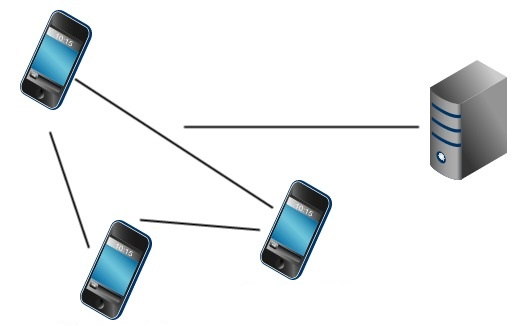
\includegraphics[width=0.4\textwidth]{img/adhoc_dtn}
	\caption{Exemple de figura}
	\label{fig-exemple}
\end{figure}

\subsection{Un altre exemple de subsecció}
\label{subsec-exemple2}

La taula \ref{tab:senzilla} és un exemple de taula senzilla. En canvi, la taula \ref{tab:taula2} és més completa.

Hi ha moltes referències \textit{on-line} de \LaTeX, com \cite{latex}.

% Utilitzeu el begin table només en cas de vole taules flotants. Si les voleu al lloc, tabular directament.
\begin{table}
\caption{Taula d'exemple}
\label{tab:senzilla}
\begin{center}
\begin{tabular}{|c|c|}
\hline
One & Two\\
\hline
Three & Four\\
\hline
\end{tabular}
\end{center}
\end{table}



\begin{table}
\caption{Taula més completa}
\label{tab:taula2}

\begin{center}
\begin{tabular}{ |l|l|l| }
\hline
\multicolumn{3}{ |c| }{Team sheet} \\
\hline
Goalkeeper & GK & Paul Robinson \\ \hline
\multirow{4}{*}{Defenders} & LB & Lucus Radebe \\
 & DC & Michael Duburry \\
 & DC & Dominic Matteo \\
 & RB & Didier Domi \\ \hline
\multirow{3}{*}{Midfielders} & MC & David Batty \\
 & MC & Eirik Bakke \\
 & MC & Jody Morris \\ \hline
Forward & FW & Jamie McMaster \\ \hline
\multirow{2}{*}{Strikers} & ST & Alan Smith \\
 & ST & Mark Viduka \\
\hline
\end{tabular}
\end{center}
\end{table}

\section{Conclusions}

.... ..  .... .. .... ... ..... ... ..... ... ... ..... .... .
.... ..  .... .. .... ... ..... ... ..... ... ... ..... .... .
.... ..  .... .. .... ... ..... ... ..... ... ... ..... .... .
.... ..  .... .. .... ... ..... ... ..... ... ... ..... .... .
.... ..  .... .. .... ... ..... ... ..... ... ... ..... .... .
.... ..  .... .. .... ... ..... ... ..... ... ... ..... .... .
.... ..  .... .. .... ... ..... ... ..... ... ... ..... .... .
.... ..  .... .. .... ... ..... ... ..... ... ... ..... .... .
.... ..  .... .. .... ... ..... ... ..... ... ... ..... .... .
.... ..  .... .. .... ... ..... ... ..... ... ... ..... .... .
.... ..  .... .. .... ... ..... ... ..... ... ... ..... .... .
.... ..  .... .. .... ... ..... ... ..... ... ... ..... .... .
.... ..  .... .. .... ... ..... ... ..... ... ... ..... .... .
.... ..  .... .. .... ... ..... ... ..... ... ... ..... .... .

\section*{Agraïments}

... ..  .... .. .... ... ..... ... ..... ... ... ..... .... .
.... ..  .... .. .... ... ..... ... ..... ... ... ..... .... .
.... ..  .... .. .... ... ..... ... ..... ... ... ..... .... .
.... ..  .... .. .... ... ..... ... ..... ... ... ..... .... .
.... ..  .... .. .... ... ..... ... ..... ... ... ..... .... .

\begin{thebibliography}{11}
\bibitem{latex}
http://en.wikibooks.org/wiki/LaTeX

\bibitem{2}
Referència 2

\bibitem{3}
Etc.


\end{thebibliography}

\appendix

\section*{Apèndix}

\setcounter{section}{1}

\subsection{Secció d'Apèndix}


... ..  .... .. .... ... ..... ... ..... ... ... ..... .... .
.... ..  .... .. .... ... ..... ... ..... ... ... ..... .... .
.... ..  .... .. .... ... ..... ... ..... ... ... ..... .... .
.... ..  .... .. .... ... ..... ... ..... ... ... ..... .... .
.... ..  .... .. .... ... ..... ... ..... ... ... ..... .... .

\subsection{Secció d'Apèndix}


... ..  .... .. .... ... ..... ... ..... ... ... ..... .... .
.... ..  .... .. .... ... ..... ... ..... ... ... ..... .... .
.... ..  .... .. .... ... ..... ... ..... ... ... ..... .... .
.... ..  .... .. .... ... ..... ... ..... ... ... ..... .... .
.... ..  .... .. .... ... ..... ... ..... ... ... ..... .... .


\end{document}

